\section{Supplemental Materials}
\subsection{Representations}
\subsection{All network features are correlated with one another}\label{sec:bag-of-features-hcp}
The experiment is repeated using the binarized structural connectomes from HCP dataset. For all $1059$ connectomes, which have 70 vertices, the network features are computed. Figure \ref{fig:exp6_hcp} \textit{top row} shows the distributions for all connectomes, and \textit{middle row} and \textit{bottom row} show the distributions after constraining by considering all connectomes with number of edges between $1010$ and $1210$, and then by choosing a network with $1100$ edges at random and choosing all networks with at most $300$ edge differences. Even in real data, constraining the networks produce similar distributions of network statistics. 

\begin{figure}[b!]
    \centering
    \includegraphics[width=\textwidth]{figures/dnd/exp6_hcp.pdf}
    \caption
    [Density plots of network statistics on HCP connectomes.]
    {\textbf{Density plots of network statistics on HCP connectomes.} All connectomes ($N=1059$) have 70 vertices defined by the Deskian parcellation. 
    \textit{(Top row)} The distributions of networks statistics for all HCP connectomes are shown.
    \textit{(Middle Row)} connectomes are constrained by only considering all networks with $1100 \pm 100$ edges.
    and \textit{(Bottom Row)} A base graph with $1100$ edges is chosen at random, and only networks that have differences up to $300$ edges are considered. Similar to the simulated examples, the distributions are qualitatively similar.}
    \label{fig:exp6_hcp}
\end{figure}


\subsection{Model Extensions}\label{sec:model_extensions}
\subsubsection{Weighted Models}
The single graph models in Section \ref{sec:single_graph_models} can be extended to weighted graphs trivially. For example, in the \textit{a priori} $\sbm$, each distinct community of edges within the graph, simply take the corresponding entries of the adjacency matrix $\A_{ij}$ to take distribution $F_{ij}$ with parameters $\pmb \theta_{ij}$. Adding additional structure to $F_{ij}$ allows the parameters $\theta_{i,j}$ to be estimable for a single graph. In particular, we will be concerned with the Truncated-Normal $\sbm$, where:
\begin{align*}
    \A_{ij}; \vec\tau_i = k, \vec\tau_j = l, \pmb \theta_{kl} \overset{ind}{\sim} \tnorm (\pmb \theta_{kl})
\end{align*}
Where $\pmb \theta_{kl} = (\mu_{k,l}, \sigma^2_{k,l}, \textrm{min}_{k,l}, \textrm{max}_{k,l})$ are the parameters associated with the $k, l$ block of edge weights.

\subsubsection{Degree-Corrected Models}
In the standard $\sbm$ defined in Section \ref{sec:usbm}, the degree of a vertex, or the expected number of edges incident to a vertex, is constant within each block. Thus, vertices with same block assignment are stochastically equivalent to each other, which can limit practical applications \cite{karrer2011stochastic}. 
In $\mathsf{degree-corrected} \sbm$ ($\dcsbm$),  there is an additional ``promiscuity'' parameter that allows vertices within blocks to have heterogeneous expected degree distributions. 

Similar to the standard $\sbm$, the \textit{a priori} $\dcsbm$ is parameterized by a vertex assignment vector $\vec \tau \in \left\{1, \hdots, K\right\}^n$, a symmetric $K \times K$ block connectivity probability matrix $\B$ with entries in $[0,1]^{K \times K}$, and the degree correction (``promiscuity'') vector $\vec \theta \in\RR^n$. 
The degree correction vector is constrained such that $\sum_i^n \vec \theta_i \mathbb{I} (\tau_i=k)=1$ for $k\in[K]$ where $\mathbb{I}$ is an indicator function. 
The model is $\A\sim\dcsbm_n(\vec\tau, \B, \vec \theta)$ if $\A$ has entries $\A_{ij} \sim \bern(\vec\theta_i \vec\theta_j\B_{kl})$ where $k=\tau_i , l=\tau_j$, for $i, j \in [n]$, and $k, l \in [K]$. 
The \textit{a posteriori} $\dcsbm$ model is additionally parameterized by a block membership probability vector $\vec{\pi} = [\pi_1,\dots,\pi_K]^\top$. The model is $\A \sim \sbm_n(\vec \pi,\B, \vec \theta)$ if $\A$ has entries $\A_{ij} \big | k=\tau_i, l=\tau_j \sim \bern(\vec\theta_i \vec\theta_j\B_{kl})$, where $\tau_i {\sim} \multinomial(\vec \pi)$ for $i \in [n]$. 

\subsection{Single Graph Applications}\label{sec:single_app_appendix}
\subsubsection{Independent Edge Modelling}\label{sec:siem_wt}
In Figure \ref{fig:dros_siem}, we investigate the appropriateness of different $\siem$ for the weighted \textit{Drosophila} connectome, similar to Figure \ref{fig:siem_uwt}.  Our goal is the same as previously; ie, to identify whether within-hemisphere connectivity exceeds between-hemisphere connectivity. Figure \ref{fig:dros_siem}(A) shows a comparison of the within and the between-hemisphere edge blocks. The within-hemisphere edge blocks appear to have a higher proportion of non-zero edges than the between-hemisphere edge blocks. This effect is significant, with the interpretation that within-hemisphere connectivity exceeds between-hemisphere connectivity at $\alpha=.05$ (Mann-Whitney Wilcoxon Test, $n=103041$, $p$-value$=0.0$). Figure \ref{fig:dros_siem}(B) shows a comparison of the homotopic and heterotopic edge blocks. The homotopic edges appear to have a higher proportion of non-zero edges with smaller edge weights, and a similar proportion of non-zero edges with larger edge weights. Homotopic connectivity significantly exceeds heterotopic connectivity at $\alpha=.05$ (Mann-Whitney Wilcoxon Test,  $n=103041$, $p$-value$=0.0$).

\begin{figure}
    \centering
    \includegraphics[width=\linewidth]{figures/dnd/dros_siem.pdf}
    \caption
    [Goodness of fit of homophilic and homotopic $\siem$ for weighted \textit{Drosophila} mushroom body.]
    {\textbf{Goodness of fit of homophilic and homotopic $\siem$ for weighted \textit{Drosophila} mushroom body}. \textbf{(A)} A comparison of the homophilic communities as determined by the hemispheres of incident vertices. The relative heights of the bars are normalized by the square root of the proportion due to the fact that the substantial majority of edges in both communities have a weight of $0$. Within-hemisphere edges appear to have greater connectivity than between-hemisphere edges. Within-hemisphere edges show significantly higher connectivity than between-hemisphere edges (Mann-Whitney Wilcoxon Test, $n=103041$, $p$-value$=0.0$). \textbf{(B)} A comparison of the homotopic edge communities, where homotopic edges are those that are incident a bilateral pair of vertices. Homotopic edges appear to have greater connectivity than heterotopic edges. Homotopic connectivity significantly exceeds heterotopic connectivity (Mann-Whitney Wilcoxon Test, $n=103041$, $p$-value$=0.0$).}
    \label{fig:dros_siem}
\end{figure}

In Figure \ref{fig:siem_os_mri} we explore the appropriateness of the $\siem$ for diffusion connectomes from the HCP Dataset. Figure \ref{fig:siem_os_mri}(A) shows the average diffusion connectome over all participants in the study. Figure \ref{fig:siem_os_mri}(B) shows the distribution of edge-weights within-hemisphere versus between-hemisphere. The diffusion connectomes appear to possess homophily; ie, high within-hemisphere connectivity, with lower between-hemisphere connectivity. To test this observation, we employ the $\texttt{MWW}$ test. All $1059$ diffusion connectomes have significantly higher within-hemisphere connectivity than between-hemisphere connectivity at $\alpha=.05$ after Bonferroni correction \cite{Bonferroni1936-ip}.

\begin{figure}
    \centering
    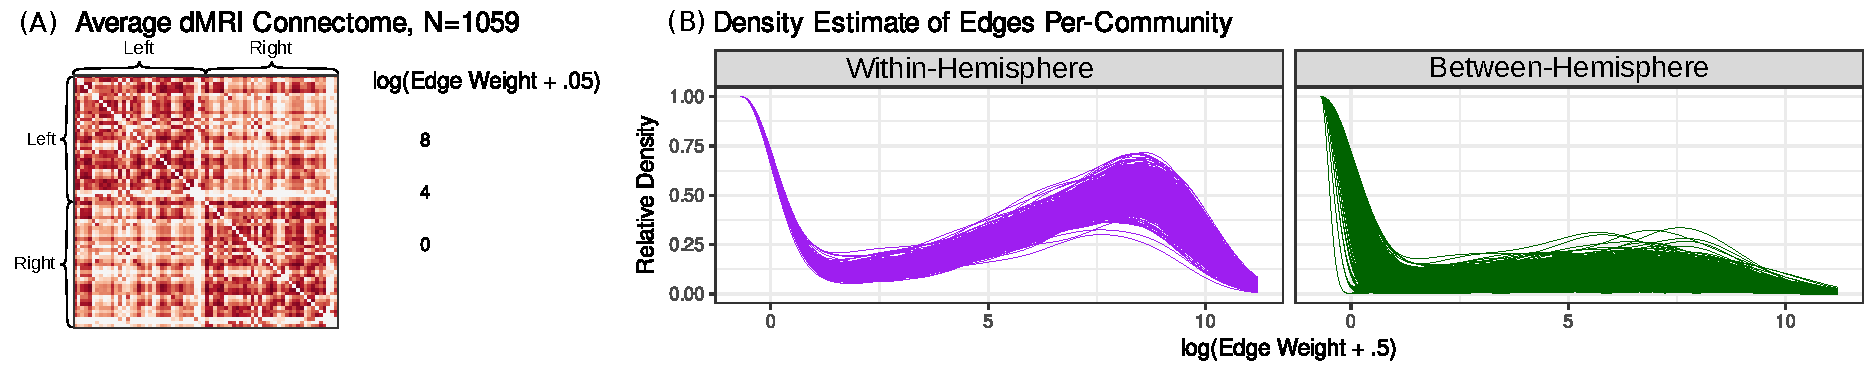
\includegraphics[width=\linewidth]{figures/dnd/hcp_siem.pdf}
    \caption
    [Goodness of fit of homophilic $\siem$ for diffusion connectomes.]
    {\textbf{Goodness of fit of homophilic $\siem$ for diffusion connectomes}. \textbf{(A)} The average diffusion connectome over $N=1059$ connectomes with $n=70$ vertices from the HCP dataset shows that diffusion connectomes appear to be homophilic, with higher within-hemisphere connectivity than between-hemisphere connectivity. Hemisphere annotations are provided for regions in the left and right hemispheres. Within-hemisphere edges are edges whose vertices are both located in the same hemisphere of the brain (the on-diagonal blocks). \textbf{(B)} Density estimates for the within-hemisphere and between-hemisphere edges for each of the $N=1059$ connectomes. Homophily is tested per-graph using the Mann-Whitney Wilcoxon Test to detect whether the on-diagonal blocks have higher connectivity than the off-diagonal blocks. All $N=1059$ diffusion connectomes have significantly higher within-hemisphere connectivity than between-hemisphere connectivity after Bonferroni correction at $\alpha=.05$, and the maximum corrected $p$-value is on the order of $10^{-21}$.}
    \label{fig:siem_os_mri}
\end{figure}

\subsubsection{Identification of Optimal Block Structure}\label{sec:sbm_est_wt}

In Figure \ref{fig:dros_sbm_est}, we investigate the appropriate block structure for the weighted \textit{Drosophila} mushroom body. \ref{fig:dros_sbm_est}(I) shows the distribution of edges associated with each block of $\B$, where the $n=319$ vertices in either the left or right hemisphere are partitioned according to hemisphere. Again, the weighted \textit{Drosophila} mushroom body is directed, so assuming symmetry would not be sensible. We investigate whether the \textit{Drosophila} mushroom body is $\er$, planted partition, symmetric heterogeneous, or asymmetric heterogeneous $\sbm$, using Kruskal-Wallis (KW), Distance Correlation (DCorr), and Analysis of Variance (ANOVA). Each method identifies the planted partition $\sbm$ as the most appropriate block model. This has the interpretation that the best-fit $\sbm$ includes a shared distribution for the on-diagonal (Left,Left) and (Right,Right) blocks, and a different shared distribution for the off-diagonal (Left,Right) and (Right,Left) blocks. An important considerations is that while the best-fit $\sbm$ is symmetric, the graph itself is directed. This has the implication that while the best-fit $\sbm$ would posit that edges in the (Left,Right) and (Right,Left) blocks have the same distribution, realizations of the (Left,Right) and (Right,Left) block will not necessarily be identical.

\begin{figure}
    \centering
    \includegraphics[width=.8\linewidth]{figures/dnd/dros_sbm_est.pdf}
    \caption
    [Identifying the appropriate block structure of the \textit{Drosophila} mushroom body.]
    {\textbf{Identifying the appropriate block structure of the \textit{Drosophila} mushroom body}. We investigate the appropriate block structure in the \textit{Drosophila}  mushroom body, with $n=319$ vertices in the left or right hemisphere. Each block corresponds to the proportion of edges with the listed edge weight. As in Figure \ref{fig:dros_siem}, the proportion of edges are shown on a scale in which bar height corresponds to the square root of the proportion, due to the presence of a large number of zero-weight edges. We investigate whether the $\sbm$ is $\er$, planted partition, symmetric heterogeneous, or asymmetric heterogeneous $\sbm$, using Kruskal-Wallis (KW), Distance Correlation (DCorr), and Analysis of Variance (ANOVA) for model selection. All approaches identify planted partition $\sbm$ as the best-fit block structure.}
    \label{fig:dros_sbm_est}
\end{figure}

In Figure \ref{fig:nested_sbm_ts_mri}, we investigate the appropriate block structure for diffusion connectomes, analogous to the single graph investigations using the \textit{Drosophila} mushroom body in Figure \ref{fig:dros_sbm_est}. Panel \textbf{(A)} demonstrates the distribution of edges associated with each block of $\B$. Panel \textbf{(B)} shows the fraction of diffusion connectomes that accept each of the candidate hypotheses, using $3$ different approaches for weighted graph model selection: Kruskal-Wallace  \cite{Kruskal1952-kj}, Distance Correlation (Dcorr) \cite{Szekely2007-mm}, and Ananysis of Variance (ANOVA) \cite{Fisher1925-xm,Scheffe1999-pi}. Diffusion connectomes tend to display planted partition structure across all model selection approaches.

\begin{figure}
    \centering
    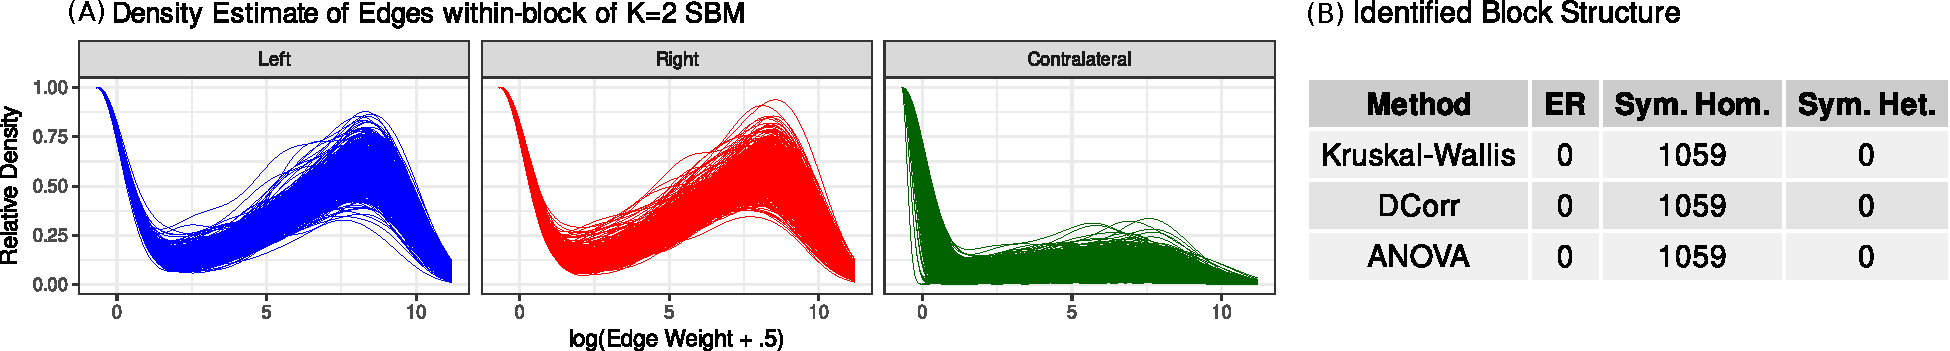
\includegraphics[width=\linewidth]{figures/dnd/hcp_block_est.pdf}
    \caption
    [Identification of appropriate block structure in diffusion connectomes.]
    {\textbf{Identification of appropriate block structure in diffusion connectomes}. We investigate the appropriate block structure in the diffusion connectomes from the HCP Dataset, with $n=70$ vertices, and $N=1059$ graphs. \textbf{(A)} the empirical distribution of edges for each of the $4$ blocks of edges for each between and within-hemisphere pair for the left and right hemispheres respectively. As the diffision connectomes are inherently symmetric, the off-diagonal blocks are inherently symmetric. The hypothesized models are that the graph is $\er$, planted partition $\sbm$ (Plant Part.), or the symmetric heterogeneous $\sbm$ (Sym. Het.). \textbf{(B)} The number of connectomes from the dataset for which the specified candidate model is selected. All methods for selection of optimal block structure identify diffusion connectomes as planted partition $\sbm$, which has the interpretation that the optimal structure is to assume that the on-diagonal left and right blocks share a common distribution that differs from the off-diagonal contralateral blocks. This conclusion holds across all diffusion connectomes within the dataset.}
    \label{fig:nested_sbm_ts_mri}
\end{figure}

\subsection{Multiple Graph Applications}\label{sec:multi_app_appendix}

\subsubsection{Testing for Significant Edges in Weighted Networks} \label{sec:exp2}
We consider two populations of networks generated from a 2 block $\sbm$, except edges are now sampled from truncated normal distribution to emulate correlation matrices. All networks have $n=20$ vertices and $\vec{\pi} = \bracks*{0.25, 0.75}$. The block edge distribution matrices for each population is given by
\begin{align*}
    \B^{(1)} &= 
    \begin{bmatrix}
        \tnorm(0, 0.25, -1, 1)   & \tnorm(0, 0.25, -1, 1) \\
        \tnorm(0, 0.25, -1, 1)   & \tnorm(0, 0.25, -1, 1) 
    \end{bmatrix} \\
    \B^{(2)} &= 
    \begin{bmatrix}
        \tnorm(0 + \delta, 0.25 + \phi, -1, 1)   & \tnorm(0, 0.25, -1, 1) \\
        \tnorm(0, 0.25, -1, 1)   & \tnorm(0, 0.25, -1, 1) 
    \end{bmatrix}
\end{align*}
where $\tnorm(\mu, \sigma^2, a, b)$ denotes a truncated normal distribution with mean $\mu$ and variance $\sigma^2$ such that all values are in $[a, b]$. Total of $m$ networks are sampled ($m/2$ networks per population). One population has the same edge weight distribution for all edges, and the second population's first block edges has either a different mean, $\delta$, or variance, $0.25 + \phi$.
For each edge, test statistics are computed with three different tests: 1) t-test, 2) Mann-Whitney (MW) U test, which is a non-parametric test of medians, and 3) two-sample Kolomogrov-Smirnov (KS) test, which is test of two distributions. Similar to experiment 1, the test statistics are sorted to find the ten most significant edges, and the performance is evaluated with recall.

Figure \ref{fig:exp2} shows the results by varying the sample size, mean, and variance. Figure \ref{fig:exp2} top row shows that all three tests can identify edges that are different in means, and that no particular test is superior than another. 
%Even at low sample sizes ($m=100$), all three tests can perfectly identify significant edges At effect size as low as $\delta = 0.3$ with sample size $m=1000$.
Figure \ref{fig:exp2} bottom row shows that only KS test can detect changes in variance when the means are kept the same. This is because t-test and MW test ultimately test for differences in centrality (e.g. mean or median), where as KS tests for any differences between a pair of observed distributions. 
% but large samples size ($m=1000$) and large effect size ($\phi\geq 2.5$) are required for high recall. 

\begin{figure}
    \includegraphics[width=.9\textwidth]{figures/dnd/exp2_change_mean}
    \includegraphics[width=.9\textwidth]{figures/dnd/exp2_change_vars}
    \caption
    [Performance of finding significant edges that have different weight distributions.]
    {\textbf{Performance of finding significant edges that have different weight distributions.}
    Recall@10 for each edge when comparing two populations of weighted networks using t-test, Mann-Whitney, and Kolmogorov-Smirnov tests. The color bar represents recall averaged over 100 trials. 
    \textit{(Top row)} Results for varying the mean $\delta$ and sample size wile keeping the variance is same ($\phi = 0$). All three tests perform equally, and can detect significant edges when edge distributions differ in means.
    \textit{(Bottom row)} Results for varying the variance $\phi$ and sample size wile keeping the mean same ($\delta = 0$). T-test and Mann-Whitney test cannot detect changes in variance regardless of the sample and effect size. KS test is the only test that can detect changes in variance.}
    \label{fig:exp2}
\end{figure}

Functional connectivity in human brains was analyzed using functional connectomes estimated using fMRI data from the HCP dataset. In functional connectomes, the edges represent correlations of changes in blood flow between a pair of ROIs, which is a proxy for correlations of brain activity. For each edge, the class-conditional mean and the variance of truncated normal distribution are computed for males ($m=330$) and females ($m=407$). Networks are then simulated as above using the 2-block weighted $\sbm$, but the parameters for first block, $\B_{11}$, is substituted with class-conditional means and variances. The performance is measured with recall@10, denoted empirical trustworthiness in Figure \ref{fig:exp2_hcp}, is measured using KS test. Again, the empirical trustworthiness shows how one can trust that the edge is truly different. There are 70 vertices with 2380 total edges, but only 256 edges have trustworthiness $\geq 0.9$.

\begin{figure}
    \centering
    \includegraphics[width=0.45\textwidth]{figures/dnd/exp2_empirical_trustworthiness}
    \caption
    [Functional connectomes are derived from the HCP data.]
    {Functional connectomes are derived from the HCP data. Vertices are defined by Desikan parcellation into 70 ROIs, and are organized by hemisphere, denoted left hemisphere (L) and right hemisphere (R). Edge weights are correlations represent correlation of brain activity between a pair of ROIs. 
    For each edge, the class-conditional means and the variances for females ($m=407$) and males ($m=330$) are computed, which are used to simulate weighted 2-block $\sbm$. Recall@10, denoted empirical trustworthiness, is measured from test statistics using KS test. Out of the 2380 total edges, only 256 edges have trustworthiness $\geq 0.9$. 
    }
    \label{fig:exp2_hcp}
\end{figure}

\subsubsection{Testing for Significant Edges Using Communities in Binary Networks} \label{sec:exp3}
In previous section \ref{sec:exp1}, the community structure was ignored even though the generative process produced two communities. In the following experiment, the community assignments are used to test whether all edges within a community or across communities are significantly different. Formally, the following hypothesis test is considered: 
\begin{align*}
    H_0:~ \PP[\B_{ij}|Y=0] = \PP[\B_{ij}|Y=1]\\
    H_A:~  \PP[\B_{ij}|Y=0]\neq \PP[\B_{ij}|Y=1]
\end{align*}
where $\PP[\B_{ij}|Y=y]$ denotes class-conditional distribution of edges that belong to community $i$ and $j$, and $i, j\in [K]$ where $K$ denotes the number of communities. When $i =j$, the edges are incident to vertices that belong to the same community. When $i\neq j$, the edges are incident to vertices that do not belong in the same community. In this setting, a total of $\frac{(K)(K+1)}{2}$ null hypothesis are tested.  

We consider two populations of networks with the connectivity probability matrices as below, 
\begin{align*}
\B^{(1)} = 
    \begin{bmatrix}
    p & p \\ p & p
    \end{bmatrix},~
\B^{(2)} = 
    \begin{bmatrix}
    p+\delta & p \\ p & p
    \end{bmatrix}
\end{align*}
with $n=50$ vertices, and membership vector, $\vec{\pi} = \bracks*{0.5, 0.5}$. Total of $m$ networks are sampled ($m/2$ networks per population). Since $K=2$, community assignment results in three sets of edges, two within communities and one across communities. The t-test statistic was computed for each set of edges, and significant edges are identified by the hypothesis test that resulted in largest test-statistic. The performance is measured by precision, which measures false positive rate, and recall, which measures true positive rate.

Figure \ref{fig:exp3} shows the results of using t-test as the effect size is changed using known and estimated community assignments. When the community assignment is known \textit{a priori}, significant edges can be perfectly detected with no false positives at low sample sizes ($m=10$) and effect size ($\delta \geq 0.05$). However, estimating community assignments results in large number of false positives edges as shown in precision plots for both $\jrdpg$ and $\cosie$ models since recovery of community assignments is correlated with magnitude of the effect size. When effect size is small, communities cannot be reliably recovered for both $\jrdpg$ and $\cosie$ models, which results in false positive tests. As effect size increases, community recovery improves and the number of false positive edges decrease at effect size ($\delta \geq 0.2$). 

\begin{figure}
    \includegraphics[width=.9\textwidth]{figures/dnd/exp3_final}
    \caption
    [Performance of finding significant edges using either known or estimated community structure.]
    {\textbf{Performance of finding significant edges using either known or estimated community structure.}
    Precision \textit{(top row)} and recall \textit{(bottom row)} for
    significant edges using t-test on sets of edges from within community or across communities averaged over 50 trials.
    \textit{(Left column)} shows the precision and recall when using true community assignments. At low sample sizes ($m =10$) and low effect size ($\delta \geq 0.05$), community wise testing results in perfect precision and recall.
    \textit{(Middle column)} shows the results for using community assignments estimated under the $\jrdpg$ model. 
    \textit{(Right column)} shows the results for using community assignments estimated under the  $\cosie$ model. 
    Since recovery of community assignment is related to the effect size, spectral clustering results in misclassified vertices. As a result, precision is low at effect sizes $\leq 0.2$. As effect size increases, the communities become more identifiable, and results in increased precision for $\jrdpg$ and $\cosie$ models. However, COSIE model requires larger effect size to reach precision $\geq 0.95$.
    }
    \label{fig:exp3}
\end{figure}

\subsubsection{Testing for Significant Edges Using Communities in Weighted Networks} \label{sec:exp4}
We consider weighted 2-block $\sbm$ similar to that of Section \ref{sec:exp2}, but with $n=50$ vertices, membership vector, $\vec{\pi} = \bracks*{0.5, 0.5}$, and block edge distribution is as below: 
\begin{align*}
    \B^{(1)} &= 
    \begin{bmatrix}
        \tnorm(0, 0.25, -1, 1)   & \tnorm(0, 0.25, -1, 1) \\
        \tnorm(0, 0.25, -1, 1)   & \tnorm(0, 0.25, -1, 1) 
    \end{bmatrix} \\
    \B^{(2)} &= 
    \begin{bmatrix}
        \tnorm(0 + \delta, 0.25 + \phi, -1, 1)   & \tnorm(0, 0.25, -1, 1) \\
        \tnorm(0, 0.25, -1, 1)   & \tnorm(0, 0.25, -1, 1) 
    \end{bmatrix}
\end{align*}
We proceed with the same experiment as that of Section \ref{sec:exp3}, while changing the means ($\delta$) or the variances ($\phi$). The community assignment is estimated using $\omni$ under $\jrdpg$ model and $\mase$ under $\cosie$ model.
The KS test statistic was computed for each set of edges, and significant edges are identified by the hypothesis test that resulted in largest test-statistic.
The performance is measured with precision and recall. 

Figure \ref{fig:exp4_means} shows the results when varying the mean ($\delta$) and Figure \ref{fig:exp4_vars} shows the results when varying the variance ($\phi$). When the community assignment is known \textit{a priori}, significant edges can be perfectly detected with no false positives at low sample sizes ($m=10$) and effect size ($\delta \geq 0.1$, $\phi \geq 0.12$). When means are changed, communities can be perfectly recovered under $\jrdpg$ model, but communities cannot be reliably recovered under $\cosie$ model. When the edge distributions are different by variance, recovering communities is impossible regardless of the statistical model. This suggest that both $\jrdpg$ and $\cosie$ models are not appropriate when studying differences in variances. 

\begin{figure}
    \centering
    \includegraphics[width=.9\textwidth]{figures/dnd/exp4_means_final.pdf}
    \caption
    [Precision \textit{(top row)} and recall \textit{(bottom row)} for significant edges using $\ks$ test averaged over 50 trials.]
    {Precision \textit{(top row)} and recall \textit{(bottom row)} for significant edges using $\ks$ test averaged over 50 trials. Effect size (x-axis) is the difference in means of the truncated normal distribution for $\B_{1, 1}$.
    \textit{(Left column)} shows the precision and recall when using known community assignments. At low sample sizes ($m =10$) and low effect size ($\delta \geq 0.1$), community wise testing results in perfect precision and recall.
    \textit{(Middle column)} shows the results for using community assignments estimated under the $\jrdpg$ model. Even at low effect size ($\delta \geq 0.15$), communities can be perfectly recovered. All significant edges can be detected without false positives. 
    \textit{(Right column)} shows the results for using community assignments estimated under the $\cosie$ model. Under this model, communities cannot be perfectly recovered, resulting in false positive edges and false negative edges.}
    \label{fig:exp4_means}
\end{figure}

\begin{figure}
    \centering
    \includegraphics[width=.9\textwidth]{figures/dnd/exp4_vars_final.pdf}
    \caption
    [Precision \textit{(top row)} and recall \textit{(bottom row)} for significant edges using $\ks$ test sets on of edges from within community or across communities averaged over 50 trials.]
    {Precision \textit{(top row)} and recall \textit{(bottom row)} for significant edges using $\ks$ test sets on of edges from within community or across communities averaged over 50 trials. Effect size (x-axis) is the difference in variances of the truncated normal distribution for $B_{1,1}$.
    \textit{(Left column)} shows the precision and recall when using known community assignments. At low sample sizes ($m =10$) and low effect size ($\phi \geq 0.12$), community wise testing results in perfect precision and recall.
    \textit{(Middle column)} shows the results for using community assignments estimated under the $\jrdpg$ model.
    \textit{(Right column)} shows the results for using community assignments estimated under the $\cosie$ model.
    Communities cannot be recovered under both $\jrdpg$ and $\cosie$ model regardless of effect size and sample size. As a result, community-wise testing result in large number of false positive edges.
    }
    \label{fig:exp4_vars}
\end{figure}

